\section{Development Environment}\label{section:development-environment2}

Section~\ref{section:development-environment1} introduced options for providing learners with programming tools and discussed their advantages and drawbacks. Subsequently, Section~\ref{section:competition} examined exemplary development tools employed in \moocs that teach programming to beginners. Based on the gained insights and the identified requirements, we decided in favor of a web-based development environment composed of a client-side code editor and a server-side component for code execution.

This approach entails a number of advantages. At first, it allows us to provide learners with a homogeneous and novice-friendly programming environment. Secondly, the approach supports a variety of programming languages and third-party libraries while providing a consistent workflow for both code execution and assessment. Thirdly, the approach enables insights into learners' problem-solving strategies by analyzing their code submissions.

\begin{figure}
\centering
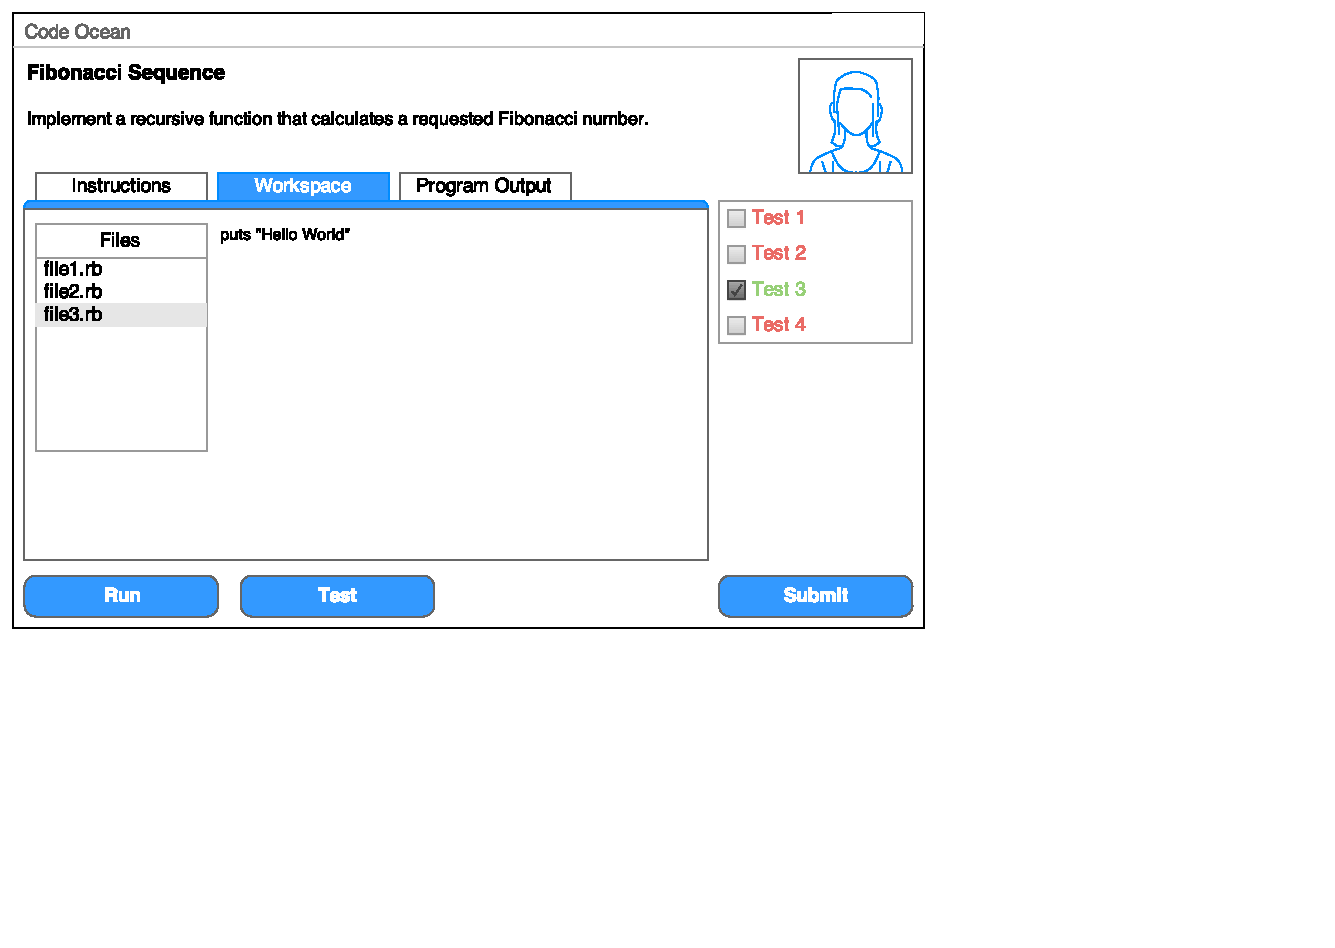
\includegraphics[clip=true, trim=0.2cm 5.4cm 6.9cm 0.2cm, width=\textwidth]{images/mockup.pdf}
\caption{Mockup of the Development Environment}
\label{figure:mockup}
\end{figure}

All web-based programming tools used in \moocs that we regarded are restricted to a single unit of editable code. In contrast, we decided that \tool should promote the concept of files. We believe that it is important to support multiple editable files and the creation of new files since this enables more profound programming exercises, fosters learners' creativity and flexibility, and empowers learners to practice program design~\cite{pieterse2013automated}.

Furthermore, we want to provide learners with the ability to explore the behavior of the code they wrote by running it as frequently as desired. In addition, code should also be assessable as frequently as demanded.

Figure~\ref{figure:mockup} depicts a mockup of a web-based development environment that incorporates our design decisions.

\tool's development environment should be based on widespread web standards that are natively supported by current web browsers. Non-native technologies, such as Java applets~\cite{truong2005learning} and third-party plugins, have to be avoided.

Currently out of scope of the web-based development environment are features for customization, debugging, and refactoring. However, we believe that the absence of these features will be negligible in the context of teaching programming to novices.
